\section{Results}
\label{sec:results}

This section presents the main CICIDS2017 results under the strict no-leakage protocol. We focus on calibrated detection performance, threshold behavior, attack-type coverage, TAD score ablation, and auditable alarm evidence. Supplementary results on SWaT and UNSW-NB15 are discussed separately and are not treated as the main evidence chain.

Unless stated otherwise, the threshold used in this section is selected only from independent benign calibration windows and then applied unchanged to the test split. Test labels are used only after threshold fixation to compute evaluation metrics.

Rather than increasing the number of loosely comparable baselines or datasets, our evaluation is organized around protocol-consistent evidence: calibrated baseline comparison, operating-point sweep, attack-family breakdown, score ablation, faithfulness sanity check, fixed-threshold sensitivity, and bounded supplementary transfer checks.

\begin{table*}[t]
  \centering
  \caption{Evaluation matrix under protocol-consistent evidence organization.}
  \label{tab:evaluation_matrix}
  \small
  \resizebox{\textwidth}{!}{%
  \begin{tabular}{p{0.23\textwidth}p{0.33\textwidth}p{0.14\textwidth}p{0.24\textwidth}}
    \toprule
    Component & Purpose & Dataset(s) & Output \\
    \midrule
    Strict compact baseline comparison & Compare representative baselines under identical strict protocol & CICIDS2017 & AUC/AP, Test FPR, P/R/F1 \\
    Operating-point sweep & Select calibrated operating point with explicit FPR trade-off & CICIDS2017 & target\_fpr vs observed Test FPR + F1 \\
    Attack-type breakdown & Expose attack-family coverage and failure mode boundaries & CICIDS2017 & Recall@\(\tau\) and mean fused score \\
    TAD score ablation & Quantify critic-only, feature-only, and fused score trade-off & CICIDS2017 & Test FPR, P/R/F1, AUC/AP \\
    IG masking faithfulness & Check whether attribution-ranked evidence affects score more than random masking & CICIDS2017 & IG vs random score-drop summary \\
    Single-window alarm trace & Provide case-level score-to-evidence-to-decision audit path & CICIDS2017 & case figure + masking decision flip \\
    Fixed-threshold sensitivity & Assess ranking-vs-threshold behavior under perturbation & CICIDS2017 & AUC/AP and Test FPR@\(\tau\), P/R/F1@\(\tau\) \\
    Supplementary ICS validation & Provide bounded transfer evidence outside main chain & SWaT & Ours + baseline supplementary metrics \\
    Distribution-shift stress test & Expose threshold-transfer limitation under shift & UNSW-NB15 & Ours + baseline supplementary metrics \\
    \bottomrule
  \end{tabular}
  }
\end{table*}


\subsection{Main CICIDS2017 Detection Results}

Table~\ref{tab:compact_baselines} reports the main CICIDS2017 comparison. The proposed method achieves AUC 0.9783 and AP 0.9631. At the selected calibrated operating point, it obtains observed test benign FPR 0.0460, precision 0.9384, recall 0.9568, and F1 0.9475.

Compared with the representative strict-protocol baselines, the proposed method provides the strongest balance between alert noise and attack coverage. GANomaly reaches F1 0.8490, but its recall is lower at 0.8276. TranAD obtains observed FPR 0.0864, but recall is 0.6321. The MLP baseline produces a substantially higher observed FPR of 0.3663. IsolationForest and OneClassSVM perform poorly in this strict window-level setting.

These results suggest that the proposed detector is most useful when evaluated as a calibrated alarm generator rather than only as a ranking model. AUC and AP indicate score separability, while the selected operating point shows how this separability translates into a concrete test-time threshold with low observed benign FPR. In other words, we evaluate both \emph{ranking quality} and \emph{alarm policy quality}: a detector can rank well yet still be operationally noisy if threshold calibration is not independently controlled.

\begin{table*}[!t]
  \centering
  \caption{CICIDS2017 strict compact baseline comparison under a unified no-leakage protocol.}
  \label{tab:compact_baselines}
  \small
  \begin{tabular*}{\textwidth}{@{\extracolsep{\fill}}lcccccc@{}}
    \toprule
    Method & AUC & AP & Test FPR & Precision & Recall & F1 \\
    \midrule
    Ours & 0.9783 & 0.9631 & 0.0460 & 0.9384 & 0.9568 & 0.9475 \\
    MLP & 0.7499 & 0.8312 & 0.3663 & 0.5908 & 0.7220 & 0.6498 \\
    GANomaly & 0.9338 & 0.8660 & 0.0893 & 0.8716 & 0.8276 & 0.8490 \\
    TranAD & 0.8431 & 0.7984 & 0.0864 & 0.8428 & 0.6321 & 0.7224 \\
    IsolationForest & 0.4053 & 0.5043 & 0.3839 & 0.4204 & 0.3801 & 0.3992 \\
    OneClassSVM & 0.6043 & 0.4487 & 0.3406 & 0.5172 & 0.4981 & 0.5075 \\
    \bottomrule
  \end{tabular*}
\end{table*}


\subsection{Threshold Sweep}

Table~\ref{tab:threshold_sweep} reports the effect of different calibration target FPR values. The target-FPR field in this sweep is a calibration-side threshold-selection parameter derived from independent benign calibration windows, not the deployed benign alarm rate. At target FPR 0.15 and 0.20, the observed benign FPR is low, but recall remains limited at 0.4627 and 0.5490. At the selected target FPR 0.25, recall increases to 0.9568 while the observed benign FPR remains 0.0460. At target FPR 0.30, recall further increases to 0.9824, but the observed benign FPR rises to 0.1134.

Among the evaluated calibration targets, target FPR 0.25 is reported as the selected operating point because, under strict independent calibration, it provides high recall while keeping the observed benign false-positive rate below 5\% on this split. We include neighboring calibration targets to show the sensitivity of the alarm trade-off, rather than to imply test-set threshold tuning. We emphasize that this does not mean the system ``allows 25\% benign false alarms'' in deployment; the deployment-facing quantity is observed test benign FPR after threshold fixation.

\begin{table}[!t]
  \centering
  \caption{Threshold sweep under strict independent benign calibration. The selected operating point is target\_fpr=0.25.}
  \label{tab:threshold_sweep}
  \small
  \resizebox{\columnwidth}{!}{%
  \begin{tabular}{cccccc}
    \toprule
    target\_fpr & Test FPR & Precision & Recall & F1 & Selected \\
    \midrule
    0.1500 & 0.0105 & 0.9700 & 0.4627 & 0.6265 & No \\
    0.2000 & 0.0158 & 0.9621 & 0.5490 & 0.6991 & No \\
    0.2500 & 0.0460 & 0.9384 & 0.9568 & 0.9475 & Yes \\
    0.3000 & 0.1134 & 0.8638 & 0.9824 & 0.9193 & No \\
    \bottomrule
  \end{tabular}
  }
\end{table}


\subsection{Attack-Type Breakdown}

Table~\ref{tab:attack_breakdown} reports performance by attack type at the selected fixed threshold \(\tau=0.425420\). To improve interpretability beyond recall alone, the table also reports attack share, Missed windows (FN), Miss Rate, score distribution (mean/median), and score-to-threshold gap. The detector performs well on Distributed Denial-of-Service (DDoS) and PortScan windows, with Recall@\(\tau\) of 0.9650 and 0.9642, respectively, and positive average score gaps above \(\tau\). These two attack types account for most anomalous windows and largely explain the strong aggregate recall.

However, the detector fails on Bot windows in this configuration. The Bot category contains 148 windows, and none are detected at the selected threshold (FN=148, Miss Rate=1.0000). Its Avg Anomaly Score is 0.2673, yielding a negative score gap of \(-0.1581\) relative to \(\tau=0.425420\).

This failure is an important limitation and a useful boundary signal. A plausible explanation is that Bot windows are relatively fewer in this split, and their behavioral signatures may be weaker than the high-intensity DDoS/PortScan patterns that dominate the calibrated operating point. With one global fixed threshold, calibration can bias toward stronger and higher-volume anomaly patterns, leaving weaker families under-detected.

The aggregate CICIDS2017 result should therefore not be interpreted as uniform attack-family coverage. The current operating point is effective for dominant DDoS/PortScan categories, while Bot remains uncovered at this threshold. This motivates attack-family-aware calibration, adaptive thresholding, or multi-threshold policy design in future work.

For metric scope, AUC/AP in Table~\ref{tab:compact_baselines} remain global ranking metrics over all test windows. We do not report per-family precision/F1 in this table because benign false positives are generated from one shared benign pool under a single global threshold; naively assigning those false positives to attack families would introduce denominator ambiguity and can be misleading.

\begin{table*}[t]
  \centering
  \caption{Attack-type breakdown at the selected fixed threshold \(\tau=0.425420\) (target\_fpr \(=0.25\)). Attack Share gives each family's proportion among anomalous test windows. Recall@\(\tau\) and Miss Rate are fixed-threshold detection and miss ratios. Avg/Median Anomaly Score summarize pre-threshold fused TAD anomaly scores per family. Score Gap indicates whether a family is, on average, above (\(>0\)) or below (\(<0\)) the alarm threshold.}
  \label{tab:attack_breakdown}
  \small
  \resizebox{\textwidth}{!}{%
  \begin{tabular}{lccccccccc}
    \toprule
    Attack Type & Total & Attack Share (\%) & Detected (TP) & Missed (FN) & Recall@\(\tau\) & Miss Rate & Avg Anomaly Score & Median Anomaly Score & Score Gap to \(\tau\) \\
    \midrule
    Bot & 148 & 0.80 & 0 & 148 & 0.0000 & 1.0000 & 0.2673 & 0.2771 & -0.1581 \\
    DDoS & 8117 & 43.73 & 7833 & 284 & 0.9650 & 0.0350 & 0.5691 & 0.5117 & +0.1437 \\
    PortScan & 10297 & 55.47 & 9928 & 369 & 0.9642 & 0.0358 & 0.4993 & 0.4939 & +0.0739 \\
    \bottomrule
  \end{tabular}
  }
  \vspace{4pt}
  \parbox{\textwidth}{\small \textit{Note:} \(\text{Score Gap to }\tau = \text{Avg Anomaly Score} - \tau\). Positive values indicate the family mean is above the alarm threshold; negative values indicate it is below.}
\end{table*}


\subsection{TAD Score Ablation}

Table~\ref{tab:tad_ablation} reports the TAD score ablation. The critic-only variant obtains observed FPR 0.0591, precision 0.9125, recall 0.8419, F1 0.8758, AUC 0.9536, and AP 0.9509. The feature-deviation-only variant is stronger, obtaining observed FPR 0.0496, precision 0.9337, recall 0.9536, F1 0.9436, AUC 0.9768, and AP 0.9616.

The fused score with $\alpha=0.24$ obtains the best calibrated trade-off: observed FPR 0.0460, precision 0.9384, recall 0.9568, F1 0.9475, AUC 0.9783, and AP 0.9631.

This ablation indicates that feature deviation is the dominant individual signal in the current configuration. The critic contributes complementary information, but the improvement from fusion is modest. Therefore, we do not claim that the adversarial component alone explains the performance. The evidence supports a more conservative conclusion: the calibrated fusion of critic evidence and benign-reference deviation provides the best operating point among the evaluated variants.

\begin{table}[t]
  \centering
  \caption{TAD score ablation under identical strict calibration settings (target\_fpr=0.25).}
  \label{tab:tad_ablation}
  \small
  \resizebox{\columnwidth}{!}{%
  \begin{tabular}{lcccccc}
    \toprule
    Score Mode & Test FPR & Precision & Recall & F1 & AUC & AP \\
    \midrule
    critic\_only & 0.0591 & 0.9125 & 0.8419 & 0.8758 & 0.9536 & 0.9509 \\
    feature\_deviation\_only & 0.0496 & 0.9337 & 0.9536 & 0.9436 & 0.9768 & 0.9616 \\
    fused (\(\alpha=0.24\)) & 0.0460 & 0.9384 & 0.9568 & 0.9475 & 0.9783 & 0.9631 \\
    \bottomrule
  \end{tabular}
  }
\end{table}


\subsection{Auditable Alarm Evidence}

Table~\ref{tab:xai_faithfulness} reports a lightweight auditability check based on attribution-guided masking. Integrated Gradients masking produces larger score drops than random masking across the evaluated masking sizes. At $k=5$, the average IG score drop is 0.0742, compared with 0.0281 for random masking. At $k=20$, the IG drop increases to 0.0950, while the random drop is 0.0269. IG masking beats random masking in 90.62\% of evaluated cases at $k=20$.

These results indicate that the attribution signal is related to the detector score. We interpret this experiment as post-hoc evidence localization and a masking-based decision check for analyst audit traces: highlighted time-feature regions have a stronger effect on alarm scores than random regions.

\begin{table}[t]
  \centering
  \caption{IG masking faithfulness summary on correctly detected anomalous windows (strict CICIDS2017 case set).}
  \label{tab:xai_faithfulness}
  \scriptsize
  \resizebox{\columnwidth}{!}{%
  \begin{tabular}{cccccc}
    \toprule
    k & Orig. & IG Drop & Rand. Drop & $\Delta$Drop & IG$>$Rand \\
    \midrule
    5 & 0.5172 & 0.0742 & 0.0281 & 0.0461 & 0.7656 \\
    10 & 0.5172 & 0.0742 & 0.0233 & 0.0509 & 0.8438 \\
    20 & 0.5172 & 0.0950 & 0.0269 & 0.0682 & 0.9062 \\
    \bottomrule
  \end{tabular}
  }
\end{table}


\subsection{Single-Window Alarm Trace}

We inspect one DDoS alarm to illustrate a concrete audit path using the correlation-pruned non-redundant feature view. The selected case has index 13570, fused score 0.506530, threshold \(\tau=0.425420\), and benign-reference mean 0.3361. Since the case score exceeds \(\tau\), the window is reported as an alarm.

The top IG-ranked time steps are 43, 39, 35, 40, and 36, indicating that the attribution mass is concentrated around a local temporal region of the window.

Attention weights are available for this case, and the top-10 overlap between attention and IG time steps is 3/10. This partial overlap suggests that attention and IG provide related but not identical views of the alarm evidence.

The top IG-ranked features in the correlation-pruned non-redundant view are Bwd Packet Length Std, PSH Flag Count, URG Flag Count, Idle Min, SYN Flag Count, Bwd IAT Total, Destination Port, Flow IAT Mean, Min Packet Length, and FIN Flag Count. These features provide a less repetitive evidence summary by reducing strongly correlated packet-length variants.

Correlation pruning here is used only to reduce repetitive evidence display based on feature correlation. It is not a proof of statistical independence.

Figure~\ref{fig:case_attribution_heatmap_main} localizes case-level evidence in a time-feature heatmap where rows are correlation-pruned non-redundant features ranked by mean absolute IG and columns are window time steps.

\begin{figure*}[t]
  \centering
  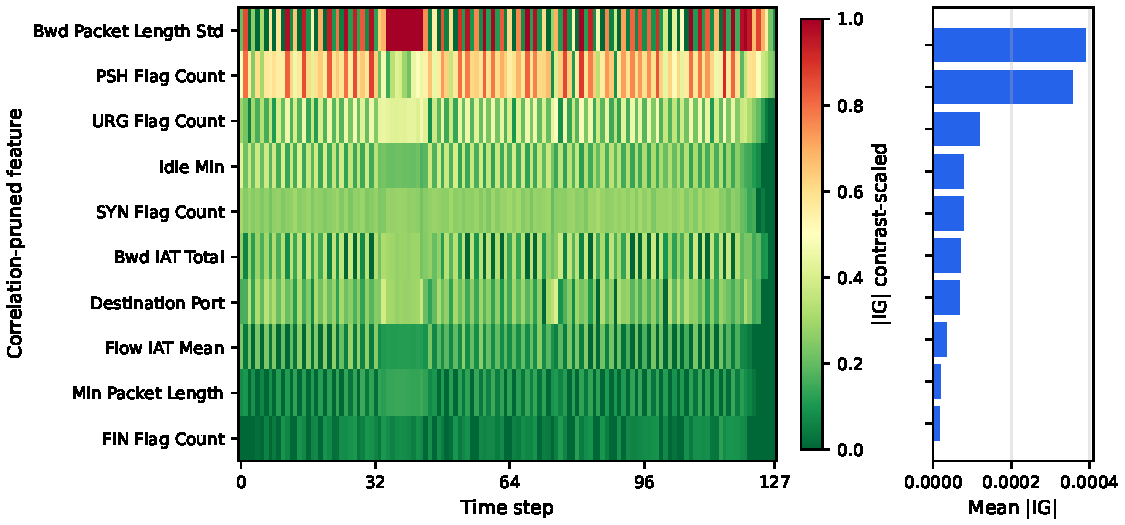
\includegraphics[width=0.96\textwidth]{figures/case_trace_attribution_heatmap_mainpaper.pdf}
  \Description{Case-level attribution heatmap for a detected DDoS window, with correlation-pruned non-redundant feature rows and time-step columns, plus a side bar of mean absolute integrated gradients.}
  \caption{Case-level attribution heatmap for a detected DDoS window. The case fused score is 0.506530, above the fixed threshold \(\tau=0.425420\); the benign-reference mean score is 0.3361. Rows show correlation-pruned non-redundant features ranked by mean absolute Integrated Gradients, and columns show time steps within the window. Correlation pruning is used only to reduce repetitive evidence display, not to establish statistical independence.}
  \label{fig:case_attribution_heatmap_main}
\end{figure*}

Masking provides a decision-level audit check. Figure~\ref{fig:case_masking_main} shows that masking top IG-ranked positions at $k=10$ and $k=20$ reduces the fused score below \(\tau\), flipping the decision to no alarm, while random masking remains above \(\tau\). This case provides an analyst-facing audit trace from score, to localized evidence, to masking-based decision change.

\begin{figure}[t]
  \centering
  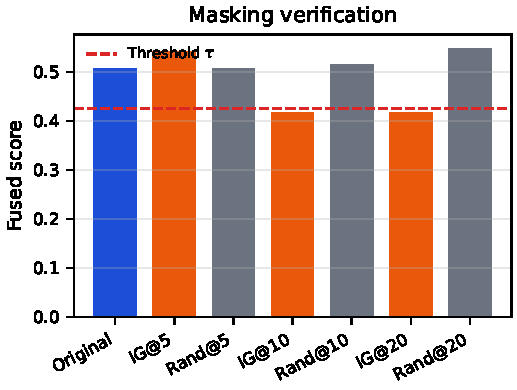
\includegraphics[width=\columnwidth]{figures/case_trace_masking_mainpaper.pdf}
  \Description{Masking-based decision verification for the selected DDoS case at fixed threshold tau; IG-guided masking at k=10 and k=20 falls below threshold while random masking stays above threshold.}
  \caption{Masking-based decision verification for the same DDoS case. The threshold \(\tau=0.425420\) is fixed. Masking top IG-ranked positions at \(k=10\) and \(k=20\) reduces the fused score below \(\tau\) and flips the decision to no alarm, while random masking remains above \(\tau\).}
  \label{fig:case_masking_main}
\end{figure}

\subsection{Fixed-Threshold Sensitivity Analysis}

Table~\ref{tab:noise_sensitivity} reports fixed-threshold sensitivity under Gaussian perturbation. Mild perturbation (\(\sigma=0.01\)) has limited effect on ranking performance, with AUC decreasing from 0.978349 to 0.977773 and AP decreasing from 0.963120 to 0.961328. However, fixed-threshold alarm metrics degrade under stronger perturbations. At \(\sigma=0.03\), Test FPR@\(\tau\) rises to 0.352003 and F1@\(\tau\) drops to 0.802693. At \(\sigma=0.05\), Test FPR@\(\tau\) rises to 0.963568 and F1@\(\tau\) drops to 0.603198.

The apparently counter-intuitive combination of high AUC/AP and high Test FPR@\(\tau\) is expected in this fixed-threshold sensitivity setting. AUC/AP summarize score ranking over possible thresholds, while Test FPR@\(\tau\) measures benign alarms at the clean-calibrated threshold. Under stronger perturbations, benign scores shift upward and many benign windows cross \(\tau\), causing high false positives. Attack scores can still remain ranked above benign scores on average, preserving AUC/AP. This indicates threshold miscalibration under perturbation rather than a contradiction between the metrics.

\begin{figure*}[t]
  \centering
  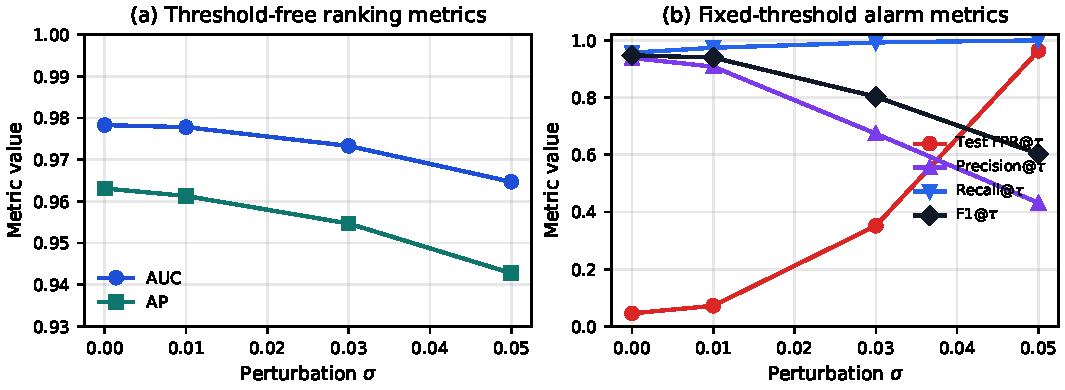
\includegraphics[width=0.96\textwidth]{figures/fixed_threshold_sensitivity_mainpaper.pdf}
  \Description{Two-panel trend plot under Gaussian perturbation: threshold-free ranking metrics AUC/AP and fixed-threshold metrics Test FPR at tau, precision at tau, recall at tau, and F1 at tau.}
  \caption{Fixed-threshold sensitivity under Gaussian input perturbation. The threshold \(\tau=0.425420\) is selected on the clean independent benign calibration split and then kept fixed for all perturbed test evaluations. AUC/AP decrease gradually, while Test FPR@\(\tau\) rises sharply and F1@\(\tau\) declines, indicating threshold miscalibration under perturbation.}
  \label{fig:fixed_threshold_sensitivity}
\end{figure*}

These results should be interpreted cautiously. The ranking quality is relatively stable under mild perturbation, but the calibrated threshold is not robust to larger distribution changes. Therefore, we do not claim strong robustness. In deployment, threshold calibration would need monitoring and possible recalibration when benign traffic changes.

\subsection{Supplementary Cross-Dataset Results}

Supplementary results on SWaT and UNSW-NB15 are reported as bounded transfer checks, not as co-equal evidence chains. Table~\ref{tab:cross_dataset_supplementary} summarizes the strict-protocol cross-dataset view with role annotations and the operating-point policy used for supplementary rows.

\begin{table*}[t]
  \centering
  \caption{Strict-protocol cross-dataset summary. CICIDS2017 is reported at the selected main operating point from the calibration sweep, while SWaT and UNSW-NB15 are reported at a fixed supplementary target\_fpr=0.05 to avoid dataset-specific favorable target selection; these rows are not intended as a direct cross-dataset ranking table.}
  \label{tab:cross_dataset_supplementary}
  \small
  \resizebox{\textwidth}{!}{%
  \begin{tabular}{llcccccccc}
    \toprule
    Dataset & Role & target\_fpr & AUC & AP & Test FPR & Precision & Recall & F1 & Interpretation \\
    \midrule
    CICIDS2017 & Primary calibrated evidence & 0.25 & 0.978349 & 0.963120 & 0.046023 & 0.938395 & 0.956847 & 0.947531 & Primary evidence \\
    SWaT & Supplementary ICS validation & 0.05 & 0.990444 & 0.997744 & 0.000000 & 1.000000 & 0.989982 & 0.994966 & Supplementary ICS check \\
    UNSW-NB15 & Distribution-shift stress test & 0.05 & 0.806125 & 0.754875 & 0.027463 & 0.240964 & 0.007032 & 0.013666 & Threshold-transfer failure \\
    \bottomrule
  \end{tabular}
  }
\end{table*}


SWaT is used as supplementary industrial-control validation. Table~\ref{tab:swat_supplementary_baselines} reports strict-protocol baseline comparison at target\_fpr=0.05; Ours reaches AUC 0.9904, AP 0.9977, Test FPR 0.0000, Precision 1.0000, Recall 0.9900, and F1 0.9950, providing supportive supplementary industrial-control evidence under the same calibration discipline. We interpret this as bounded evidence under one ICS setting, not as comprehensive validation across industrial-control environments.

\input{tables/table_swat_supplementary_baselines.tex}

UNSW-NB15 is treated as a distribution-shift stress test. Ours has non-trivial ranking (AUC 0.8061, AP 0.7549) but very low calibrated recall (0.0070) with F1 0.0137 at target\_fpr=0.05. This gap between ranking and thresholded recall indicates that a benign-calibrated threshold transferred from a different regime can fail even when score ordering remains partially informative. We therefore interpret UNSW-NB15 as explicit failure-mode evidence for threshold transfer, not as a success case.

The MLP row in the UNSW supplementary baseline table is a supervised window-label reference, whereas Ours and the anomaly baselines operate under benign-window anomaly-detection assumptions. Additional UNSW baseline details are kept as supplementary artifact material to preserve the main-text focus on the CICIDS2017 primary evidence chain.

For operating-point sensitivity outside CICIDS2017, we retain the strict two-point supplementary comparison (target\_fpr 0.05 and 0.15) as artifact-level evidence only; we do not present it as a full threshold sweep in the main text.

\subsection{Summary of Findings}

The CICIDS2017 strict-protocol results support three main findings. First, the proposed detector provides a strong calibrated operating point, achieving high recall and F1 while keeping observed benign FPR below 5\% on the test split. Second, the TAD score is most effective as a fused calibrated score, with feature deviation serving as the dominant signal and the critic adding complementary information. Third, the detector can provide auditable alarm evidence through time-step attribution, feature attribution, and masking-based decision checks.

At the same time, the results expose important limitations. Bot attacks are missed at the selected threshold. Fixed-threshold behavior is sensitive to stronger perturbations. Supplementary UNSW-NB15 results show very low recall under distribution shift, exposing a threshold-transfer limitation. These limitations motivate future work on attack-family-aware calibration, adaptive thresholding, and broader validation under realistic traffic shifts.
